\documentclass[border=4pt]{standalone}
\usepackage{pgfplots}
\usepgfplotslibrary{fillbetween}
\pgfplotsset{compat=1.18}

\begin{document}
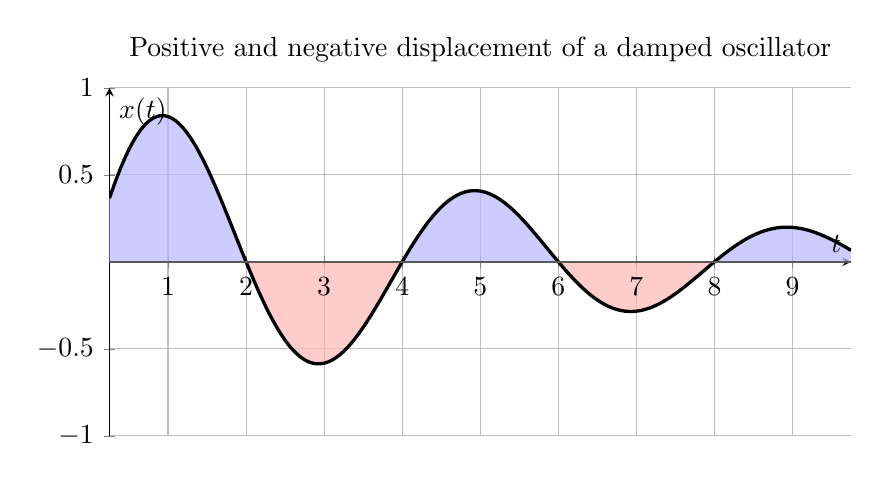
\begin{tikzpicture}
  \begin{axis}[
    width=11cm,
    height=6cm,
    xmin=0.25,
    xmax=9.75,
    ymin=-1,
    ymax=1,
    axis lines=middle,
    grid=major,
    xlabel={$t$},
    ylabel={$x(t)$},
    title={Positive and negative displacement of a damped oscillator}
  ]
    \addplot[
      name path=signal,
      black,
      very thick,
      domain=0.25:9.75,
      samples=191
    ] {exp(-0.18*x)*sin(90*x)};
    \addplot[
      name path=zero,
      gray!70!black,
      thick,
      domain=0.25:9.75,
      samples=2
    ] {0};
    \addplot[fill=blue!28,fill opacity=0.72] fill between[
      of=signal and zero,
      split,
      every even segment/.style={fill=blue!28},
      every odd segment/.style={fill=red!28}
    ];
  \end{axis}
\end{tikzpicture}
\end{document}
